\chapter{TSP Approximation}
\label{chapter:tsp}

A well recognized problem in combinatoral optimisation is the Travelling Salesman Problem (TSP). It is usually presented in a practical form: given a list of $n$ cities and distances between them, find the shortest route that visits each city exactly one time and returns to the origin city \cite{kruskal1956shortest}. Such problem is NP-hard, although very useful in many practical cases.

Any TSP problem can be converted into QAP, thus TSP can be though as speciaisation of Quadratic Assignment Problem. To do such conversion TSP distance matrix can be used without any changes as QAP distance matrix, while QAP flow matrix is filled with same constant values.

Introduced in this thesis Physarum-based Metaheuristic is a method of looking through the space search and it is not dependant on any specific problem. As such it can be used with ease for other problems than QAP --- a definition of neighbourhood and cost function is required. As a example, we made simplified tests of the algorithm, approximating TSP tour.


\section*{Implementation}

While any instance of TSP could be tread as an instance of QAP, we preffered to create a speciaised implementation of \texttt{Problem} class, as it need not to store any flow values. A \texttt{TspProblem} has been created, which defines $cost$ as sum of distances between each of cities in the tour. The same neighbourhood as in QAP is used: a single pair swap in a tour, creating neighbourhood of size $\frac{n\cdot(n-1)}{2}$ for every possible tour.

An input format is simplier than with QAP, as only single matrix needs to be provided --- first line of input contains size of the problem $n$, followed by $n{\times}n$ numbers representing the distance matrix. Output is defined as in QAP --- the problem size $n$, followed by total distances $f$, followed by $n$ numbers representing the tour (rearranged so it starts with city numbered one).

Using \texttt{build.sh} script, executable files \texttt{bin/physarum-tsp} and \texttt{bin/physarum-tsp-debug} can be created. Configuration options are the same as with QAP version (table \ref{table:pi_options}).


\section*{Results}

Test dataset is a subset of TSPLIB, which is library containing multiple instances of synthetic and practical problem definitions with optimal tours \cite{reinhelt2014tsplib}. Data from the TSPLIB has been preprocessed to be compliant with the input format.

In comparison to QAP use case, it has been observed that larger values of $E_{explore}$ are preffered (figure \ref{figure:tsp_explore_frontier}). Using large values of $E_{explore}$ forces the plasmodium to preffer deeper crawling than local exploration. Furthermore, usage of $E_{explore}=0.01$ gives plasmodium the most energy, even though less solutions are explored (figure \ref{figure:tsp_explore_energy}).

\begin{figure}
  \centering

  \includegraphics[width=1.1\textwidth,center]{algorithm/metaheuristic/charts/tsp/u/tsp_explore_frontier.\eop}

  \caption{Cost of the best detected solution with different explore energy $E_{explore}$ (dataset \texttt{berlin52})}
  \label{figure:tsp_explore_frontier}
\end{figure}

\begin{figure}
  \centering

  \includegraphics[width=1.1\textwidth,center]{algorithm/metaheuristic/charts/tsp/u/tsp_explore_energy.\eop}

  \caption{Plasmodium energy $E_{plasmodium}$ with different explore energy $E_{explore}$ (dataset \texttt{berlin52}, $q=10$, $a=0.1$)}
  \label{figure:tsp_explore_energy}
\end{figure}

However, it could be seen that usage of default exponential base $q=10$ and scaling factor $a=0.1$ in cost-to-food transformation makes energy vary very much with each epoch. This is subefficient behaviour and should be controlled --- providing too much energy for mildly better solution causes the plasmodium to stay for longer in local minima neighbourhood. THe neighbourhood in TSP is characterised differently than in QAP, even a small change can result in large change of tour length. Different scaling factor has been tested and rather smaller values of $q$ (and $a=\frac{1}{q}$) are preffered (figure \ref{figure:tsp_ctf_energy}). As result of choosing smaller values of exponential base $q$, the algorithm behaves less erratically, finding better solutions (figure \ref{figure:tsp_ctf_frontier}). 

\begin{figure}
  \centering

  \includegraphics[width=1.1\textwidth,center]{algorithm/metaheuristic/charts/tsp/u/tsp_ctf_energy.\eop}

  \caption{Plasmodium energy $E_{plasmodium}$ with different exponential base $q$ (dataset \texttt{berlin52}, $a=\frac{1}{q}$)}
  \label{figure:tsp_ctf_energy}
\end{figure}

\begin{figure}
  \centering

  \includegraphics[width=1.1\textwidth,center]{algorithm/metaheuristic/charts/tsp/u/tsp_ctf_frontier.\eop}

  \caption{Cost of the best detected solution with different exponential base $q$ (dataset \texttt{berlin52}, $a=\frac{1}{q}$)}
  \label{figure:tsp_ctf_frontier}
\end{figure}

Considered TSP instances are rather large, therefore using large number of initial samples $k$ is recommended (figure \ref{figure:tsp_samples_cost}). Colony of virtual plasmodium is started on better solutions, requiring less epochs for being close to optimum.

\begin{figure}
  \centering

  \includegraphics[width=1.1\textwidth,center]{algorithm/metaheuristic/charts/tsp/u/tsp_samples_cost.\eop}

  \caption{Cost of the best detected solution with different number of initial samples $k$ (dataset \texttt{berlin52}, $q=1.25$, $a=0.8$, $E_{explore}=0.01$, $l=10$)}
  \label{figure:tsp_samples_cost}
\end{figure}

Even though rather large values of $E_{explore}$ are preffered for algorithm stabilisation, when using large number of samples $k=1000000$, initial solution can be quite close to the optimum, therefore exploring their local neighbourhood thoroughly could result in finding even better solutions at initial epochs. 

In order to allow such behaviour, some initial energy $E_{initial}$ must be introduced, so more exhaustive exploration phase can be done even the same $E_{explore}$ is used. Selecting a rather large $E_{initial}=100$ allows for exploring extra $10000$ neighbour solutions (when $E_{explore}=0.01$), resulting with better overall results (figure \ref{figure:tsp_initial_cost}).

\begin{figure}
  \centering

  \includegraphics[width=1.1\textwidth,center]{algorithm/metaheuristic/charts/tsp/u/tsp_initial_cost.\eop}

  \caption{Cost of the best detected solution with different initial energy $E_{initial}$ (dataset \texttt{berlin52}, $q=1.25$, $a=0.8$, $E_{explore}=0.01$, $l=10$, $k=1000000$)}
  \label{figure:tsp_initial_cost}
\end{figure}

\section*{Conclusion}

Usage the Physarum-based Metaheuristic for approximating tours of Travelling Salesman Problem required different tuning of the algorithm as the problem has much different characterstics than QAP. Using the parameters that have been chosen experimentally (scaling factor $a=0.8$, exponential base $q=1.25$, $E_{explore}=0.01$, $l=10$, $k=1000000$, $E_{initial}=100.0$, $E_{crawl}=0.001$), tests have been performed on subset of instances varying in size from the \texttt{TSPLIB}. In total tests have been performed ten times for each instance, time limited to $t=10n$, but no longer than 3600~s. Aggregated results in form of distance to optimal length are provided in figure \ref{figure:tsp_final}.

\begin{figure}
  \centering

  \includegraphics[width=0.9\textwidth]{algorithm/metaheuristic/charts/tsp/final/distance.eps}

  \caption{Aggregated results for various TSP instances}
  \label{figure:tsp_final}
\end{figure}

In the end it can be seen, that can be seen that proposed algorithm behaves quite well on multiple datasets, yielding results at most $10\%$ worse than optimal tours, however on some datasets approximated tour are far from optimal and cannot be considered useful. Some further work is needed in order to make use of Physarum-based Metaheuristic for reliable approximation of TSP tours.
